\documentclass[10pt, letterpaper]{paper}
\usepackage{graphicx}
\usepackage{amsmath}
\usepackage{float}

\title{ Operations Research HW3 }
\author{ Timothy Schwieg }
\date{ September 22 2017 }

\begin{document}

\maketitle

\section*{Question 1 }

\begin{equation*}
\begin{alignedat}{3}
&\text{max }&3x_1 + x_2&\\
&\text{s.t. } &4x_1 + x_2  &\geq 4\\
& &2x_1 + x_2  &\leq 4\\
& &x_1 + x_2 &= 3\\
& &x_1, x_2, x_3, s_1, s_2, a_1 &\geq 0
\end{alignedat}
\end{equation*}

\subsection*{a.}
\begin{figure}[h!]
\centering
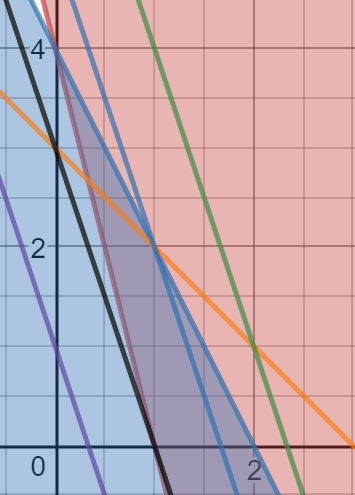
\includegraphics[width=0.4\textwidth]{desmos-graph__3_.png}
\caption{ Feasible set and level sets }

%Graph Here
\end{figure}
Note that the orange line is a constraint.
%Graph Stuff here

\subsection*{b.}
\begin{equation*}
\begin{alignedat}{10}
&Z &- 3x_1 &- x_2 &  & &-Ma_1 &-Ma_3&= 0\\
& &4x_1 &+ x_2 &-s_1 & &+a_1 & &=4\\
& &2x_1 &+ x_2 & &+s_2 & &  &= 4\\
& &x_1 &+ x_2 & & & &+a_3 &= 3\\
\end{alignedat}
\end{equation*}

Putting it into Clean Table form
\[
	\left[ {\begin{array}{ccccccc|c}
	Z & x_1 & x_2 & s_1 & s_2 & a_1 & a_2 & RHS\\ \cline{1-8}
	1 & -3 - 5M & -1 - 2M & M & M & 0 & 0 &-7M \\
	0 & 4 & 1 & -1 & 0 & 1 & 0 & 4 \\
	0 & 2 & 1 & 0 & 1 & 0 & 0 & 4 \\
	0 & 1 & 1 & 0 & 0 & 0 & 1 & 3  \\
	\end{array} } \right]
\]

\[
	\left[ {\begin{array}{ccccccc|c}
	Z & x_1 & x_2 & s_1 & s_2 & a_1 & a_2 & RHS\\ \cline{1-8}
	1 & 0 & \frac{-1 - 3m}{4} & \frac{-3-M}{4} & M & \frac{3+5M}{4} & 0 &3-2M \\
	0 & 1 & \frac{1}{4} & \frac{-1}{4} & 0 & \frac{1}{4} & 0 & 1 \\
	0 & 0 & \frac{1}{2} & \frac{1}{2} & 1 & \frac{-1}{2} & 0 & 2  \\
	0 & 0 & \frac{3}{4} & \frac{1}{4} & 0 & \frac{-1}{4} & 1 & 2  \\
	\end{array} } \right]
\]

\[
	\left[ {\begin{array}{ccccccc|c}
	Z & x_1 & x_2 & s_1 & s_2 & a_1 & a_2 & RHS\\ \cline{1-8}
	1 & 0 & 0 & \frac{-2}{3} & M & \frac{2+3M}{3} & \frac{1+3M}{3} & \frac{11}{3} \\
	0 & 1 & 0 & \frac{-1}{3} & 0 & \frac{1}{3} & \frac{-1}{3} & \frac{1}{3} \\
	0 & 0 & 0 & \frac{1}{3} & 1 & \frac{-1}{3} & \frac{-2}{3} & \frac{2}{3}  \\
	0 & 0 & 1 & \frac{1}{3} & 0 & \frac{-1}{3} & \frac{4}{3} & \frac{8}{3}  \\
	\end{array} } \right]
\]


\[
	\left[ {\begin{array}{ccccccc|c}
	Z & x_1 & x_2 & s_1 & s_2 & a_1 & a_2 & RHS\\ \cline{1-8}
	1 & 0 & 0 & 0 & M+ 2 & M & M - 1 & 5 \\
	0 & 1 & 0 & 0 & 1 & 0 & -1 & 1 \\
	0 & 0 & 0 & 1 & 3 & -1 & -2 & 2  \\
	0 & 0 & 1 & 0 & -1 & 0 & 2 & 2  \\
	\end{array} } \right]
\]

From here we can see that $x_1$ = 1, $x_2$ = 2, $s_1$ = 2, and the maximum obtained is 5.

\subsection*{c.}

At the start of the algorithm, $s_1, a_2, a_2$ are in the basis, and  our solution is not feasible, with objective value 0. This corresponds to the origin on the graph.
\newline\newline

After One step, $x_1, s_2, a_2$ are in the basis. Since $x_1$ = 1, our solution is still not feasible, it corresponds to being along the x-axis on the graph, and the objective value is -3.
\newline\newline

After the second step, $x_1, x_2, s_2$ are in the basis, but we are still not at a feasible solution, since $x_1 + x_2 \neq 3$. The objective value is $\frac{11}{3}$
\newline\newline

At the final step, $x_1, x_2, s_1$ are in the basis, and we are finally at a feasible solution. The objective function value is 5, and on the graph we correspond to the maximum shown. 

\subsection*{d.}
We can see that the problem is not unbounded, as there are no negative elements on the Z-row with a DNE or negative minimum ratio-test. The problem is feasible because there is no artificial variables present in the basis at the final solution. 

\section*{Question 2.}
\subsection*{a.}
\begin{equation*}
\begin{alignedat}{3}
&\text{min }&4x_1 + 4x_2 + x_3&\\
&\text{s.t. } &x_1 + x_2 +x_3 &\leq 2\\
& &2x_1 + x_2  &\leq 3\\
& &2x_1 + x_2 + 3x_3 &\geq 3\\
& &x_1, x_2, x_3 &\geq 0
\end{alignedat}
\end{equation*}
This statement is equivalent to: 
\begin{equation*}
\begin{alignedat}{3}
&\text{max }&-4x_1 - 4x_2 - x_3 -Ma_1&\\
&\text{s.t. } &x_1 + x_2 +x_3 + s_1 &= 2\\
& &2x_1 + x_2 + s_2  &= 3\\
& &2x_1 + x_2 + 3x_3 - s_3 + a_1 &= 3\\
& &x_1, x_2, x_3 &\geq 0
\end{alignedat}
\end{equation*}

\[
	\left[ {\begin{array}{cccccccc|c}
	Z & x_1 & x_2 & x_3 & s_1 & s_2 & s_3 & a_1 & RHS\\ \cline{1-9}
	1 & 4 - 2M & 4- M & 1 - 3M & 0 & 0 & -M & 0 & -3M \\
	0 & 1 & 1 & 1 & 1 & 0 & 0 & 0 & 2 \\
	0 & 2 & 1 & 0 & 0 & 1 & 0 & 0 & 3  \\
	0 & 2 & 1 & 3 & 0 & 0 & -1 & 1 & 3  \\
	\end{array} } \right]
\]

\[
	\left[ {\begin{array}{cccccccc|c}
	Z & x_1 & x_2 & x_3 & s_1 & s_2 & s_3 & a_1 & RHS\\ \cline{1-9}
	1 & \frac{10}{3} & \frac{11}{3} & 0 & 0 & 0 & \frac{1}{3} & \frac{-1}{3} +M & -1 \\
	0 & \frac{1}{3} & \frac{2}{3} & 0 & 1 & 0 & \frac{1}{3} & \frac{-1}{3} & 1 \\
	0 & 2 & 1 & 0 & 0 & 1 & 0 & 0 & 3  \\
	0 & \frac{2}{3} & \frac{1}{3} & 1 & 0 & 0 & \frac{-1}{3} & \frac{1}{3} & 1  \\
	\end{array} } \right]
\]

Thus the maximum of -Z is -1, and the minimum of Z is 1. Occurring where $x_1 = 0, x_2 = 0, x_3 = 1$.

\subsection*{b.}
The problem is not infeasible as there is are no artificial variables that are still in the basis, only the slack variables.

\section*{Question 3.}
\begin{equation*}
\begin{alignedat}{3}
&\text{max }&x_1 + 2x_2&\\
&\text{s.t. } &-x_1 + x_2 &\leq 2\\
& &-2x_1 + x_2 &\leq 1\\
& &x_1, x_2 &\geq 0
\end{alignedat}
\end{equation*}
\subsection*{a.}
\begin{figure}[h!]
\centering
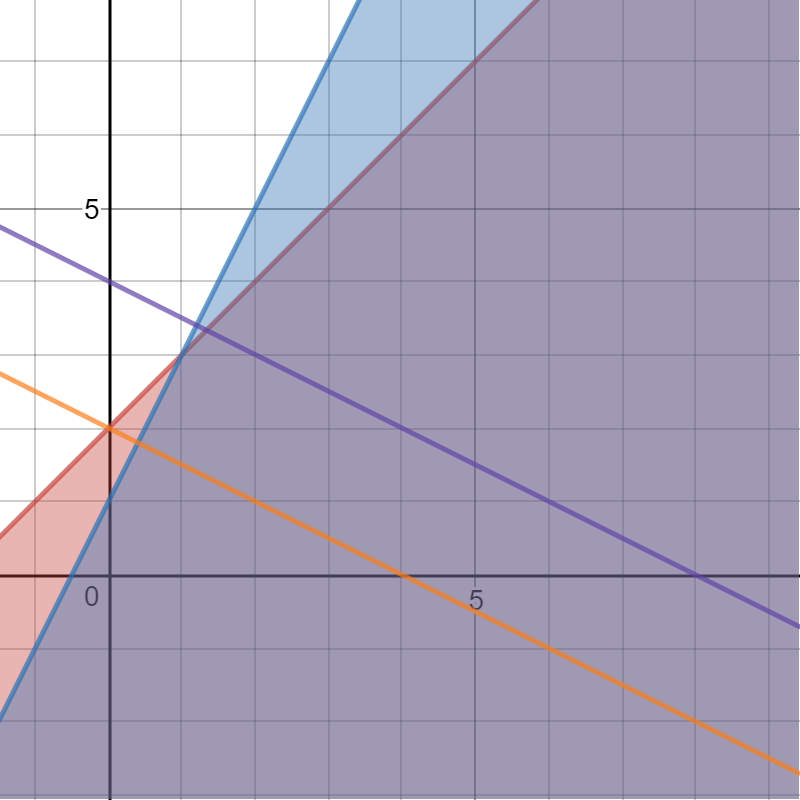
\includegraphics[width=0.4\textwidth]{desmos-graph__1_.png}
\caption{ Feasible set with Level Sets }
%Graph Here
\end{figure}
It is clear from the graph that the linear program is unbounded, as the feasible region is not bounded, and level sets can be continued on infinitely increasing the maximal value.
\subsection*{b.}
\begin{equation*}
\begin{alignedat}{3}
&\text{max }&x_1 +2x_2&\\
&\text{s.t. } &-x_1 + x_2 + s_1 &= 2\\
& &-2x_1 + x_2 + s_2  &= 1\\
& &x_1, x_2, s_1, s_2 &\geq 0
\end{alignedat}
\end{equation*}

\[
	\left[ {\begin{array}{ccccc|c}
	Z & x_1 & x_2 & s_1 & s_2 & RHS\\ \cline{1-6}
	1 & -1 & -2 & 0 & 0 & 0 \\
	0 & -1 & 1 & 1 & 0 & 2 \\
	0 & -2 & 1 & 0 & 1 & 1 \\
	\end{array} } \right]
\]

\[
	\left[ {\begin{array}{ccccc|c}
	Z & x_1 & x_2 & s_1 & s_2 & RHS\\ \cline{1-6}
	1 & -5 & 0 & 0 & 2 & 2 \\
	0 & 1 & 0 & 1 & -1 & 1 \\
	0 & -2 & 1 & 0 & 1 & 1 \\
	\end{array} } \right]
\]

\[
	\left[ {\begin{array}{ccccc|c}
	Z & x_1 & x_2 & s_1 & s_2 & RHS\\ \cline{1-6}
	1 & 0 & 0 & 5 & -3 & 7 \\
	0 & 1 & 0 & 1 & -1 & 1 \\
	0 & 0 & 1 & 2 & -1 & 3 \\
	\end{array} } \right]
\]

\subsection*{c.}
In the final tableau we can see that we would like $s_2$ to enter the basis, but the ratio for both rows is negative. This indicates that the program is unbounded, and the objective function can be made as large as possible.

\subsection*{d.}

Examining the two constraints:
\newline
$x_1 + s_1 - s_2 = 1$
\newline
$x_2 + 2s_1 - s_2 = 3$
\newline
Note that $s_2$ is what we want to enter the basis, so $s_1$ will remain 0.
\newline
$x_1 = 1 + s_2$ and $x_2 = 3 + s_2$
\newline
Thus  $\textbf{x} = {1 \choose 3} + s_2 {1 \choose 1}$ and the direction of unboundedness is: ${1 \choose 1}$

\section*{Question 4}
\subsection*{a.}
\begin{figure}[H]
\centering
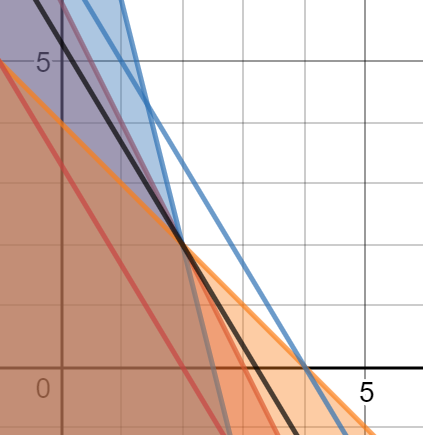
\includegraphics[width=0.6\textwidth]{desmos-graph__4_.png}
\caption{ Feasible set and level sets }

%Graph Here
\end{figure}
\subsection*{b.}
\begin{equation*}
\begin{alignedat}{3}
&\text{max }&5x_1 +3x_2&\\
&\text{s.t. } &4x_1 + 2x_2 + s_1 &= 12\\
& &4x_1 + x_2 + s_2  &= 10\\
& &x_1 + x_2 + s_3 &= 4
& &x_1, x_2, s_1, s_2, s_3 &\geq 0
\end{alignedat}
\end{equation*}

\[
	\left[ {\begin{array}{cccccc|c}
	Z & x_1 & x_2 & s_1 & s_2 & s_3 & RHS\\ \cline{1-7}
	1 & -5 & -3 & 0 & 0 & 0 & 0 \\
	0 & 4 & 2 & 1 & 0 & 0 & 12 \\
	0 & 4 & 1 & 0 & 1 & 0 & 10 \\
	0 & 1 & 1 & 0 & 0 & 1 & 4 \\
	\end{array} } \right]
\]

\[
	\left[ {\begin{array}{cccccc|c}
	Z & x_1 & x_2 & s_1 & s_2 & s_3 & RHS\\ \cline{1-7}
	1 & 0 & \frac{-7}{4} & 0 & \frac{5}{4} & 0 & \frac{25}{2} \\
	0 & 0 & 1 & 1 & -1 & 0 & 2 \\
	0 & 1 & \frac{1}{4} & 0 & \frac{1}{4} & 0 & \frac{5}{2} \\
	0 & 0 & \frac{3}{4} & 0 & \frac{-1}{4} & 1 & \frac{3}{2} \\
	\end{array} } \right]
\]

\[
	\left[ {\begin{array}{cccccc|c}
	Z & x_1 & x_2 & s_1 & s_2 & s_3 & RHS\\ \cline{1-7}
	1 & 0 & 0 & \frac{7}{4} & \frac{-1}{2} & 0 & 16 \\
	0 & 0 & 1 & 1 & -1 & 0 & 2 \\
	0 & 1 & 0 & \frac{-1}{4} & \frac{1}{2} & 0 & 2 \\
	0 & 0 & 0 & \frac{-3}{4} & \frac{1}{2} & 1 & 0 \\
	\end{array} } \right]
\]

\[
	\left[ {\begin{array}{cccccc|c}
	Z & x_1 & x_2 & s_1 & s_2 & s_3 & RHS\\ \cline{1-7}
	1 & 0 & 0 & \frac{1}{4} & 0 & 2 & 16 \\
	0 & 0 & 1 & \frac{-1}{2} & 0 & 2 & 2 \\
	0 & 1 & 0 & \frac{1}{2} & 0 & -1 & 2 \\
	0 & 0 & 0 & \frac{-3}{2} & 1 & 2 & 0 \\
	\end{array} } \right]
\]

We can see that a maximum of 16 is obtained at: $x_1 = 2,x_2 = 2, s_3 = 2,x_3=s_1=s_2 =0$ 

\subsection*{c.}
The Algorithm begins at the origin with the point: (0,0,12,10,4), it then moves to $(\frac{5}{2}, 0, 0, 2, 0, \frac{3}{2})$ found along the x-axis. After this $x_2$ enters the basis and the algorithm moves to: $(2,2,0,0,0)$ This corresponds to the maximum on the graph. The final step remains here.   


\subsection*{d.}
Yes the LP is degenerate. Notice in the second tableau there is two options of equal ratio, meaning that one constraint is redundant, and the linear program is degenerate. 

\subsection*{e.}
The linear program is not unbounded since we can see that there are no negative elements in the Z row. Since we do not see a nonbasic variable become zero in the Z row, we can conclude that there are not multiple solutions.


\section*{Question 5.}
\begin{equation*}
\begin{alignedat}{3}
&\text{max }&3x_1 +2x_2&\\
&\text{s.t. } &2x_1 + x_2 + s_1 &= 100\\
& &4x_1 + x_2 + s_2  &= 80\\
& &x_1 + s_3 &= 40\\
& &x_1, x_2, s_1, s_2, s_3 &\geq 0
\end{alignedat}
\end{equation*}

\subsection*{a.}
The new Tableau is: 

\[
	\left[ {\begin{array}{ccccccc|c}
    & 1 & d_1 & d_2 & 0 & 0 & 0 & 0 \\
	  & Z & x_1 & x_2 & s_1 & s_2 & s_3 & RHS\\ \cline{1-8}
	1 &   1 & 0 & 0 & 1  & 1  & 0 & 180 \\
	d_1 & 0 & 1 & 0 & 1  & -1 & 0 & 20 \\
	d_2 & 0 & 0 & 1 & -1 & 2  & 0 & 60 \\
	0 &   0 & 0 & 0 & -1 & 1  & 1 & 20\\
	\end{array} } \right]
\]
The reduced cost for $s_1$ is: $1 + d_1 - d_2$
The reduced cost for $s_2$ is $1 - d_1 + 2d_2$

If only $d_1$ changes, $d_2$ is 0. 
So for $s_1, s_2$ to be feasible. $1+d_1 \geq 0$ and $ 1 - d_1 \geq 0$. This implies that: $d_1 \in [-1,1]$. This means that the basis will remain optimal as long as the coefficient of $x_1 \in [2,4]$. If the objective function coefficient becomes 3.5, the basis remains optimal, and since $x_1,x_2$ are in the basis and completely determine the maximal value, it will remain unchanged at 180.

\subsection*{b.}
If only $d_2$ changes, $d_1$ is 0.
We instead arrive at: $1 - d_2 \geq 0$ and $1 + 2d_2 \geq 0$. This implies that $d_2 \in [\frac{-1}{2},1]$ and the basis will remain optimal as long as the coefficient of $x_2 \in [\frac{3}{2}, 3]$. 

\subsection*{c.}
The RHS Tableau will be: 

\[
	\left[ {\begin{array}{ccccccc|cccc}
	  & Z & x_1 & x_2 & s_1 & s_2 & s_3 & RHS & d_1 & d_2 & d_3\\ \cline{1-11}
	 &   1 & 0 & 0 & 1  & 1  & 0 & 180& 1 & 1 & 0 \\
	 & 0 & 1 & 0 & 1  & -1 & 0 & 20 & 1 & -1 & 0 \\
	 & 0 & 0 & 1 & -1 & 2  & 0 & 60 & -1 & 2 & 0 \\
	 &   0 & 0 & 0 & -1 & 1  & 1 & 20 & -1 & 1 & 1\\
	\end{array} } \right]
\]
If only $d_1$ changes, $d_2,d_3 = 0$. Feasibility conditions are:
\begin{equation*}
\begin{alignedat}{3}
&20 + d_1  &\geq 0\\
&60 - d_1  &\geq 0\\
&20-d_1 &\geq 0
\end{alignedat}
\end{equation*}
We can see that $d_1 \in [-20,20]$. This allows for the RHS to be $\in [80,120]$. If the RHS for the first constraint changes to 90, that means $d_1 = 10$. This changes the optimal value of the objective function to: $180 + d_1 + d_2 = 190$


\section*{Question 6.}
It is equivalent to state the problem in this manner:
\begin{equation*}
\begin{alignedat}{3}
&\text{max }&4x_1 - e_1 + e_2 + e_3 - e_3&\\
&\text{s.t. } &x_1 + e_1 - e_2 &\leq 5\\
& &2x_1 + e_1 - e_2 &\leq 7\\
& &-2e_1 + 2e_2 - e_3 + e_4 &\leq -6\\
& &x_1 + e_3 - e_4 &\leq 4\\
& &-x_1 -e_3 + e_4 &\leq -4\\
& &x_1, e_1, e_2, e_3, e_4 &\geq 0
\end{alignedat}
\end{equation*}
The dual of such a problem is:
\begin{equation*}
\begin{alignedat}{3}
&\text{min }&5\lambda_1 + 7\lambda_2 - 6\lambda_3 + 4\lambda_4 -4\lambda_5&\\
&\text{s.t. } &\lambda_1 + 2\lambda_2 + \lambda_4 -\lambda_5 &\geq 4\\
& &-\lambda_1 + \lambda_2 + \lambda_3 - 2\lambda_4 &\geq -1\\
& &\lambda_1 - \lambda_2 - \lambda_3 + 2\lambda_4 &\geq 1\\
& &-\lambda_3 + \lambda_4 - \lambda_5 &\geq 1\\
& &\lambda_3 - \lambda_4 + \lambda_5 &\geq -1\\
& &\lambda_1, \lambda_2, \lambda_3, \lambda_4, \lambda_5 &\geq 0
\end{alignedat}
\end{equation*}
Note that I elected to change the equality constraint to two constraints instead of allowing a dual variable to become unrestricted. I also forced all constraints in the primal to be $\leq$ so that all the constraints in the dual would be $\geq$. It is possible to form the dual without these changes, however my answer is equivalent, and follows the procedure burned into me by the math department. 



\section*{Question 7.}

\begin{equation*}
\begin{alignedat}{3}
&\text{max }&3x_1 + 4x_2 + x_3 + 5x_4&\\
&\text{s.t. } &x_1 + 2x_2 + x_3 + 2x_4 &\leq 5\\
& &2x_1 + 3x_2 + x_3 + 3x_4 &\leq 8\\
& &x_1, x_2, x_3, x_4, &\geq 0
\end{alignedat}
\end{equation*}
This problem has a dual of: 

\begin{equation*}
\begin{alignedat}{3}
&\text{min }&5\lambda_1 + 8\lambda_2&\\
&\text{s.t. } &\lambda_1 + 2\lambda_2 &\geq 3\\
& &2\lambda_1 + 3\lambda_2 &\geq 4\\
& &\lambda_1 + \lambda_2 &\geq 1\\
& &2\lambda_1 + 3\lambda_2 &\geq 5\\
& &\lambda_1, \lambda_2 &\geq 0
\end{alignedat}
\end{equation*}

\subsection*{b.}
By inspection we may note that constraint 2 is irrelevant, and that $\lambda_1 = 1, \lambda_2 = 1$ is the smallest values we may achieve. This gives us a minimum of: 13

\subsection*{c.}
Via Complementarity Slackness: $ (c- A^T \lambda )^T x = 0$ This amounts to: 

\[
	\left( \left[ {\begin{array}{c}
	3 \\
	4 \\
	1 \\
	5  \\
	\end{array} } \right] - \left[ {\begin{array}{c}
	3 \\
	5 \\
	2 \\
	5  \\
	\end{array} } \right] \right)^T \textbf{x}
    = 
    \left[ {\begin{array}{c}
	0 \\
	-1 \\
	-1 \\
	0  \\
	\end{array} } \right]^T \textbf{x} =
    0
\] 
Thus we can see that: $x_2, x_3 = 0$ Using $(b - Ax)^T \lambda = 0$ tells us that the first two constraints must bind, as both $\lambda_1$ and $\lambda_2$ are positive. Using the constraints to form a linear system we arrive at: 
\begin{equation*}
\begin{alignedat}{3}
& x_1 + 2x_4 &= 5 \\
& 2x_1 + 3x_4 &= 8\\
\end{alignedat}
\end{equation*}

This has a solution of $x_1 = 1, x_4 = 2$. Thus the maximum is: 13 at: $(1,0,0,2)$

\section*{Question 8.}
\subsection*{a.}
\begin{equation*}
\begin{alignedat}{3}
&\text{max }&-3x_1 + x_2 + 2x_3 &\\
&\text{s.t. } &x_2 + 2x_3 &\leq 3\\
& &-x_1 + 3x_3 &\leq -1\\
& &-2x_1 - 3x_2 &\leq -2\\
& &x_1, x_2, x_3, &\geq 0
\end{alignedat}
\end{equation*}
We can see that the dual of this problem is: 
\begin{equation*}
\begin{alignedat}{3}
&\text{min }&3\lambda_1 - \lambda_2 - 2\lambda_3&\\
&\text{s.t. } & -\lambda_2 -2\lambda_3 &\geq -3\\
& &\lambda_1 - 3\lambda_2 &\geq 1\\
& &2\lambda_1 + 3\lambda_2 &\geq 2\\
& &\lambda_1, \lambda_2, \lambda_3 &\geq 0
\end{alignedat}
\end{equation*}

\subsection*{b.}
By Multiplying each of the constraints in the dual by -1 we arrive at this equivalent statement for the dual: 
\begin{equation*}
\begin{alignedat}{3}
&\text{min }&3\lambda_1 - \lambda_2 - 2\lambda_3&\\
&\text{s.t. } & \lambda_2 +2\lambda_3 &\leq 3\\
& &-\lambda_1 + 3\lambda_2 &\leq -1\\
& &-2\lambda_1 - 3\lambda_2 &\leq -2\\
& &\lambda_1, \lambda_2, \lambda_3 &\geq 0
\end{alignedat}
\end{equation*}
It is clear that this is the same feasible set as the primal.
\subsection*{c.}
Let F be the feasible region for both the dual and the primal.
Via weak duality: $-3x_1 + x_2 + 2x_3 \leq 3\lambda_1 -\lambda_2 - 2\lambda_3 \quad \forall x,\lambda \in F$ 
\newline
Fix $x,\lambda$ at their optimal values $x^* and \lambda^*$. 
\newline
$-3x_1^* + x_2^* + 2x_3^* \leq 3\lambda_1^* -\lambda_2^* - 2\lambda_3^*$
\newline
However since $x^* \in F$ for the dual and $\lambda^* \in F$ for the primal. We may apply weak duality for $x = \lambda^*$ and $\lambda = x^*$.
\newline
$-3\lambda_1^* + \lambda_2^* + 2\lambda_3^* \leq 3x_1^* -x_2^* - 2x_3^*$
\newline
Thus $-3\lambda_1^* + \lambda_2^* + 2\lambda_3^* = 3x_1^* -x_2^* - 2x_3^*$ and both objective functions are equal. \newline
Note also that since $(0,0,0) \in F,$
$-3x_1^* + x_2^* + 2x_3^* \leq 0$ and $-3\lambda_1^* + \lambda_2^* + 2\lambda_3^* \geq 0$ \newline
Thus: $-3\lambda_1^* + \lambda_2^* + 2\lambda_3^* = 3x_1^* -x_2^* - 2x_3^* = 0$








\end{document}